\chapter{Opis projektnog zadatka}
		

		Cilj ovog projekta je razviti programsku podršku za stvaranje web aplikacije „Parkiraj Me“ koja korisnicima omogućuje praćenje stanja parkirališnih mjesta u gradu te njihovu rezervaciju.
		Aplikacija će objedinjavati parkirališne površine diljem Zagreba svih tvrtki zainteresiranih za ponudu svojih površina putem aplikacije.
		Ovakvim rješenjem bi se uvelike olakšalo nalaženje parkirališnih mjesta u gusto naseljenim urbanim sredinama među koje se svrstaje i grad Zagreb.\\
		
		\noindent Prilikom pokretanja aplikacije prikazuje se karta s ucrtanim parkirališnim površinama koje se nalaze u blizini. Pomoću pametnih kamera se omogućuje praćenje zauzeća pojedinih parkirališnih mjesta.\\
		
		\noindent Sustav je povezan sa Google Maps uslugom, tj. pomoću toga će se korisnicima prikazivati karta i lokacije parkinga na njoj. Vezano za tu uslugu implementirana je i opcija prijedloga parkirališnih površina na temelju trenutne lokacije korisnika.\\
		\noindent Kod davanja prijedloga u situaciji kada je na geografski najbližoj lokaciji slobodan mali broj mjesta, prednost je dana sljedećoj najbližoj lokaciji s većim brojem slobodnih mjesta, jer se može dogoditi da kad vozač stigne do parkinga više nema slobodnih mjesta.\\ 
		
		
		\noindent \underbar{Neregistriranom korisniku}
		odabirom parkirališne površine prikazuju se informacije o statusu parkirališne površine:
		
		\begin{packed_item}
			\item broj slobodnih mjesta
			\item udaljenost od parking lokacije
		\end{packed_item}		
		
		\noindent Svaki punoljetni neregistrirani korisnik ima opciju registracije. Moguće se registrirati kao privatni korisnik, tj. \underbar {vozač} ili kao \underbar {tvrtka} koja nudi svoja parking mjesta na svojim parkirališnim površinama.
		
		\noindent Pri postupku registracije korisnici koji žele napraviti račun kao vozač unose slijedeće podatke: 
		
		\begin{packed_item}
			\item korisničko ime
			\item OIB
			\item Ime i prezime
			\item E-mail
			\item Registarska oznaka vozila
			\item Broj kreditne kartice
			\item Lozinku koju žele koristiti			
		\end{packed_item}
				
				
		\noindent Korisnici koji žele napraviti račun kao vlasnici parking površina unose slijedeće podatke:
		
		\begin{packed_item}
			\item OIB tvrtke
			\item Ime tvrtke
			\item Adresu sjedišta tvrtke
			\item E-mail
			\item Lozinku koju žele koristiti			
		\end{packed_item}
		
		\noindent Što se tiče samih rezervacija postoje tri opcije:
		
		\begin{packed_item}
			\item jednokratna za vremenski period kraći od 24 sata koja se mora obaviti barem 6h unaprijed
			
			\begin{packed_item}
				\item naplata u trenutku rezervacije
			\end{packed_item}
		
			\item ponavljajuća rezervacija koja mora trajati najmanje 1h i ponavljati se barem jednom tjedno tijekom mjesec dana
			
			\begin{packed_item}
				\item naplata svakih 30 dana
			\end{packed_item}
		
			\item trajna rezervacija mjesta (0-24h svaki dan na neodređeni period)
		\end{packed_item}
		
		Naplata će se vršiti po principu da korisnici plaćaju direktnom uplatom aplikaciji što je ostvareno pomoću vanjskog servisa naplate.
		Dalje se te uplate prosljeđuju vlasnicima parking lokacija.\\
		\clearpage
		
		\noindent \underbar {Vozač} ima slijedeće mogućnosti prilikom korištenja aplikacije:
		
		\begin{packed_item}
			\item rezervacija parking mjesta
			\item pregled i izmjena:
			\begin{packed_item}
				\item osobnih podataka
				\item registriranih vozila
				\item aktivnih rezervacija
			\end{packed_item}
		\end{packed_item}
			
		\noindent \underbar {Tvrtkama} se omogućuju slijedeće mogućnosti prilikom korištenja aplikacije:
		
		\begin{packed_item}
			\item pregled i izmjena:
			\begin{packed_item}
				\item osobnih podataka o računu
				\item prijavljenih parking površina
				\item postavljenih cijena rezervacija
			\end{packed_item}
		\end{packed_item}
		
			
		\noindent \underbar{Administrator}			
		je zadnji tip korisnika. Administrator sustava ima najveće ovlasti te može upravljati i računima klijenata i računima tvrtki.
		Ima mogućnost i brisanja tih računa. 
		Prilikom brisanja računa klijenata, ako ima neiskorištenih rezervacija uplata bi se refundirala za preostalo (neiskorišteno) vrijeme. 
		Prilikom brisanja računa tvrtki obrisale bi se i sve njihove parkirališne površine, a sve preostale neiskorištene rezervacije bi se otkazale i refundirale.\\
		
		\clearpage
		
		Slična implementacija lokacija na karti i prikazivanja nekih informacija o njima prikazana je na donjim slikama.\\

				%unos slike
		\begin{figure}[H]
			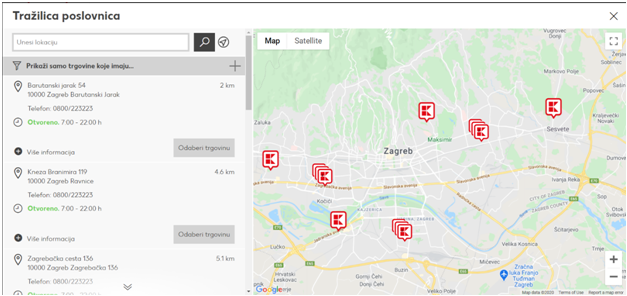
\includegraphics[scale=1]{slike/gmaps_p1.png} %veličina slike u odnosu na originalnu datoteku i pozicija slike
			\centering
			\caption{Odabir poslovnica tvrtke Kaufland,
				\url{https://www.kaufland.hr/usluge/poslovnica.html}
			}
			\label{fig:promjene}
		\end{figure}
	
				%unos slike
		\begin{figure}[H]
			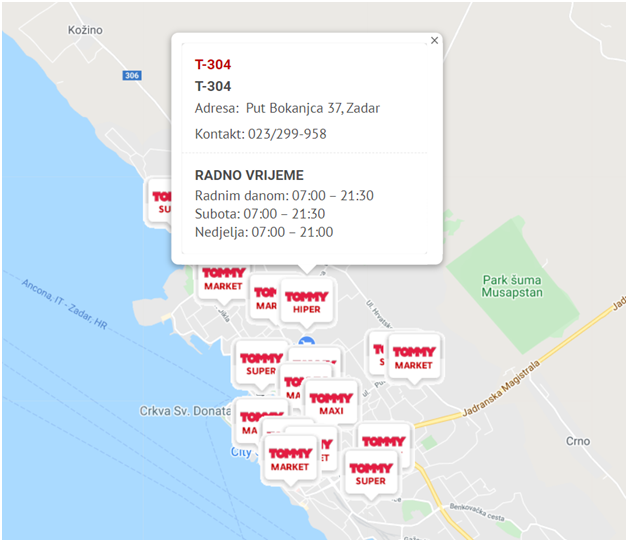
\includegraphics[scale=1]{slike/slika_2.png} %veličina slike u odnosu na originalnu datoteku i pozicija slike
			\centering
			\caption{Odabir poslovnica tvrtke Tommy,
				\url{ https://tommy.hr/hr/prodajna-mjesta}
			}
			\label{fig:promjene}
		\end{figure}

		
		\eject
		
	
